% =============================================================================
% PAT-ER MDPI Article Package
%
% Build:
%   pdflatex main.tex
%   bibtex main
%   pdflatex main.tex
%   pdflatex main.tex
%
% Primary target: Machine Learning and Knowledge Extraction (MAKE).
% To retarget, change the first documentclass option (e.g., make -> bdcc).
% =============================================================================

\documentclass[make,article,submit,pdftex,moreauthors]{Definitions/mdpi}

\firstpage{1}
\makeatletter
\setcounter{page}{\@firstpage}
\makeatother
\pubvolume{1}
\issuenum{1}
\articlenumber{0}
\pubyear{2026}
\copyrightyear{2026}
\datereceived{}
\daterevised{}
\dateaccepted{}
\datepublished{}
\doinum{}

\usepackage{mathtools}
\usepackage{tabularx}
\usepackage{booktabs}
\usepackage{multirow}
\usepackage{placeins}
\usepackage{tikz}
\usetikzlibrary{positioning, arrows.meta, calc, fit}

\def\UrlBreaks{\do\/\do-\do.\do_\do?\do\&\do\=\do\a\do\b\do\c\do\d\do\e%
  \do\f\do\g\do\h\do\i\do\j\do\k\do\l\do\m\do\n\do\o\do\p\do\q\do\r%
  \do\s\do\t\do\u\do\v\do\w\do\x\do\y\do\z\do\A\do\B\do\C\do\D\do\E%
  \do\F\do\G\do\H\do\I\do\J\do\K\do\L\do\M\do\N\do\O\do\P\do\Q\do\R%
  \do\S\do\T\do\U\do\V\do\W\do\X\do\Y\do\Z}

\newcommand{\PATER}{PAT-ER}
\newcommand{\Qwen}{Qwen3-0.6B}
\newcommand{\RtwoP}{role-to-primitive}
\newcommand{\LM}{\mathcal{L}_{\mathrm{LM}}}
\newcommand{\Laux}{\mathcal{L}_{\mathrm{aux}}}
\newcommand{\Lspan}{\mathcal{L}_{\mathrm{span}}}
\newcommand{\Liface}{\mathcal{L}_{\mathrm{iface}}}
\newcommand{\LKL}{\mathcal{L}_{\mathrm{KL}}}
\newcommand{\stopgrad}{\operatorname{sg}}
\newcommand{\Attn}{\operatorname{Attn}}
\newcommand{\LN}{\operatorname{LN}}
\newcommand{\softmax}{\operatorname{softmax}}
\newcommand{\concat}{\mathbin{\Vert}}

\Title{Primitive-Augmented Transformers with Event-Role Side State: Architecture Evidence, Warm-Started Modulation, and Decoupled Tool Interfaces}

\newcommand{\orcidauthorA}{0000-0002-5461-8899}
\newcommand{\orcidauthorB}{0000-0002-9680-2758}

\Author{Nurgali Kadyrbek $^{1,}$*\orcidA{} and Madina Mansurova $^{1}$\orcidB{}}
\AuthorNames{Nurgali Kadyrbek and Madina Mansurova}

\address{%
$^{1}$ \quad Department of AI \& Big Data, Faculty of Information Technologies, Al-Farabi Kazakh National University, Almaty 050040, Kazakhstan; Madina.Mansurova@kaznu.edu.kz}

\corres{Correspondence: kadyrbek.nurgali@kaznu.kz}


\abstract{Large language models can emit fluent text while leaving intermediate semantic structure implicit. We study whether explicit event-role and logical-primitive side-state can improve a pretrained decoder without damaging its language behavior. We introduce PAT-ER, a decoder architecture with a normal token stream, an event-role register stream, and a primitive register stream. The primitive stream is motivated by the view that logical primitives answer characteristic semantic questions, such as what licenses a conclusion, what conflicts with it, or why evidence is insufficient. Across eight seeds on the same Qwen3-0.6B backbone, replacing token-pooled auxiliary heads with typed PAT-ER registers improves primitive macro-F1 by 0.209 (95\% CI [0.182, 0.237]) and role-to-primitive macro-F1 by 0.091 (95\% CI [0.074, 0.110]) with no language-model loss cost. A generic-register control shows that this is not merely the effect of adding latent registers: typed PAT-ER improves over generic registers by 0.116 primitive macro-F1 and 0.110 role-to-primitive macro-F1, with both confidence intervals excluding zero. A warm-started model then recovers pretrained language quality (LM loss 1.344 versus 2.555 for the frozen-backbone register model) while retaining most side-state behavior. Finally, a decoupled interface mode produces robust schema-grounded function calls on 242 held-out prompts (Hermes parse 0.952, exact arguments 0.981, JSON validity 1.000, IDK F1 1.000) while base-mode side-state metrics remain byte-identical to the warm-start baseline. The model is not a theorem prover and does not achieve perfect unseen tool-name copying; the contribution is a measured architecture signal and a usable, guarded interface.}

\keyword{large language models; neural-symbolic learning; semantic roles; logical reasoning; tool use; model architecture; function calling}


\begin{document}

\section{Introduction}
\label{sec:introduction}

Transformer decoders \citep{vaswani2017attention,brown2020language} provide a
powerful token-level substrate for language modeling, but their intermediate
semantic organization is normally implicit. This is a practical problem when a
model is expected to distinguish proof from refutation, abduction from
deduction, evidence from unsupported assertion, and a safe answer from a
necessary abstention. These distinctions are not merely output labels. They are
semantic operations that structure the answer.

This paper asks whether logical primitives can be treated as \emph{semantic
heads}: fixed, named latent channels that answer characteristic questions. For
example, implication and modus ponens ask ``from what does this follow?'';
abduction asks ``what hypothesis would explain the observation?''; contradiction
asks ``what conflicts with this?''; unknown or IDK asks ``what is missing before
answering?''. The core hypothesis is architectural: if these primitives are
represented by a side-state rather than only by pooled token labels, a decoder
should learn more stable mappings between event roles, primitive class, and
output behavior.

\PATER{} (Primitive-Augmented Transformer with Event-Role Stream) implements
this hypothesis with three interacting streams:

\begin{enumerate}
  \item a standard causal token stream;
  \item an event-role stream that stores event and argument registers; and
  \item a primitive stream that stores semantic primitive registers.
\end{enumerate}

The event-role stream is grounded in linguistic work on semantic roles and
argument structure \citep{dowty1991proto,palmer2005propbank,baker1998framenet}.
The primitive stream is grounded in the use of formal reasoning labels and
proof/refutation metadata in logical NLP datasets such as ProofWriter
\citep{tafjord2021proofwriter} and FOLIO \citep{han2024folio}. The point is not
to turn a language model into a proof engine. The point is to expose a fixed
semantic flow that can be ablated, measured, and used.
This places PAT-ER inside the broader hybrid-reasoning agenda surveyed in recent
MDPI work on LLM--knowledge-graph integration and neural--symbolic reasoning
\citep{dehal2025kgllm,liang2025neurosymbolic}, but with a narrower architectural
claim: the structured state is inside the decoder rather than supplied only as
an external graph, retrieved context, or post-hoc explanation.

The experimental record supports three bounded claims. First, the register
architecture matters: on the same \Qwen{} backbone and same data, PAT-ER
registers outperform token-pooled auxiliary heads across eight seeds. Second,
the side-state can be attached to a pretrained decoder without destroying
language-model behavior, provided the injection path is register-only,
detached, and trained at a calibrated injection learning rate. Third, product
format generation can be separated from side-state measurement by a mode-gated
interface path: base mode preserves the side-state exactly, while
\texttt{interface\_mode} learns schema-grounded tool calls and JSON output.

The paper is also intentionally negative where the evidence is negative. Several
plausible paths failed: synthetic external-style augmentation hurt the real
external slice; explicit-conflict NLI hurt ProofWriter contradiction; token and
evidence-item fact heads failed at the available data scale; aux-refresh after
warm-start caused class forgetting; and shared-layer interface SFT improved tool
calls but damaged the role-to-primitive bridge. These failures are not hidden.
They are part of the method: audit, run a bounded gate, document pass and fail,
and freeze only after a pass.

\begin{figure}[H]
\centering
\resizebox{\textwidth}{!}{%
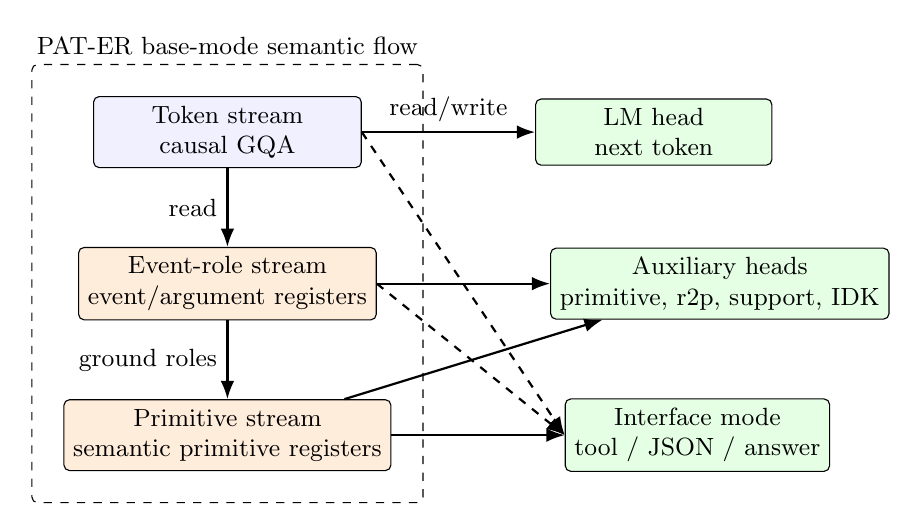
\begin{tikzpicture}[
  font=\small,
  >=Latex,
  stream/.style={draw, rounded corners=2pt, minimum width=34mm, minimum height=9mm, align=center, fill=blue!6},
  reg/.style={draw, rounded corners=2pt, minimum width=34mm, minimum height=9mm, align=center, fill=orange!14},
  head/.style={draw, rounded corners=2pt, minimum width=30mm, minimum height=8mm, align=center, fill=green!10},
  arr/.style={->, line width=0.8pt}
]
\node[stream] (tok) {Token stream\\causal GQA};
\node[reg, below=10mm of tok] (event) {Event-role stream\\event/argument registers};
\node[reg, below=10mm of event] (prim) {Primitive stream\\semantic primitive registers};
\node[head, right=22mm of event] (heads) {Auxiliary heads\\primitive, r2p, support, IDK};
\node[head, right=22mm of tok] (lm) {LM head\\next token};
\node[head, right=22mm of prim] (iface) {Interface mode\\tool / JSON / answer};

\draw[arr] (tok) -- node[above]{read/write} (lm);
\draw[arr] (tok) -- node[left]{read} (event);
\draw[arr] (event) -- node[left]{ground roles} (prim);
\draw[arr] (event) -- (heads);
\draw[arr] (prim) -- (heads);
\draw[arr] (prim) -- (iface);
\draw[arr, dashed] (event.east) -- (iface.west);
\draw[arr, dashed] (tok.east) -- (iface.west);

\node[draw, dashed, rounded corners=2pt, fit=(tok)(event)(prim), inner sep=4mm,
      label={[font=\small]above:PAT-ER base-mode semantic flow}] {};
\end{tikzpicture}%
}
\caption{PAT-ER contains a normal token stream plus event-role and primitive side-state streams. The architecture claim is evaluated in base mode. Product-format generation is handled separately by the decoupled interface path.}
\label{fig:architecture_streams}
\end{figure}



\subsection{Contributions}
\label{subsec:contributions}

This article contributes:

\begin{itemize}
  \item A semantic-head framing of logical primitives as fixed answer-structuring
  questions, implemented as a primitive side-state coupled to event-role
  registers.
  \item A decoder architecture with explicit event-role and primitive streams,
  including formulas for token/register updates, warm-start-safe injection, and
  set-valued span supervision.
  \item An eight-seed architecture matrix showing that PAT-ER registers improve
  primitive macro-F1 and role-to-primitive macro-F1 over token-pooled auxiliary
  heads on the same pretrained backbone.
  \item A warm-start procedure that preserves pretrained language behavior while
  allowing measured side-state modulation.
  \item A decoupled interface mode that produces schema-grounded tool calls and
  JSON at zero measured cost to the base-mode side-state.
\end{itemize}

\section{Related Work}
\label{sec:related}

\subsection{Transformers and Pretrained Language Models}

The Transformer architecture \citep{vaswani2017attention} replaced recurrent
sequence processing with attention over token states and remains the dominant
substrate for pretrained language models. BERT \citep{devlin2019bert} showed
the effectiveness of large-scale bidirectional pretraining for language
understanding, while GPT-style autoregressive language models demonstrated
few-shot behavior at scale \citep{brown2020language}. Parameter-efficient
adaptation methods such as LoRA \citep{hu2022lora} show that pretrained models
can often be modified without updating all backbone parameters.

PAT-ER builds on this pretrained-decoder substrate but does not treat the
decoder state as the only semantic carrier. Its central comparison is therefore
not ``pretrained versus not pretrained'', but ``token-pooled labels versus
side-state registers on the same pretrained backbone''.

\subsection{Semantic Roles and Event Structure}

Semantic-role theory studies how predicates structure their arguments. Dowty's
proto-role analysis \citep{dowty1991proto} argues that roles such as agent and
patient are better understood through clusters of entailments than through a
small rigid inventory. PropBank \citep{palmer2005propbank} and FrameNet
\citep{baker1998framenet} operationalized predicate-argument annotation for
computational NLP. These resources motivate the event-role side of PAT-ER: the
model should not only classify a primitive but also bind it to the event and
argument roles that license it.

\subsection{Logical Reasoning Benchmarks}

Natural-language reasoning datasets provide structured labels for entailment,
contradiction, and uncertainty. SNLI \citep{bowman2015snli} introduced a large
NLI benchmark with entailment, contradiction, and neutral labels. FEVER
\citep{thorne2018fever} framed fact verification as claim evaluation against
evidence. ProofWriter \citep{tafjord2021proofwriter} is closer to the present
work because it includes proofs, implications, and abductive statements over
templated natural language. FOLIO \citep{han2024folio} provides natural-language
premises with first-order logic annotations and verified reasoning labels.

PAT-ER uses these sources not to copy chain-of-thought into the input, but to
derive supervised side-state targets: primitive class, support state, rule
depth, entailment/refutation status, evidence pointers, and role-to-primitive
bridges. The no-chain-of-thought constraint is important: proof metadata is used
as supervision, not as rendered reasoning text.

\subsection{Hybrid Knowledge Extraction and Neural--Symbolic Reasoning}

Recent MDPI literature frames LLM reasoning as part of a wider effort to combine
statistical language models with structured knowledge. Dehal et al.
\citep{dehal2025kgllm} survey the reciprocal relationship between LLMs and
knowledge graphs, emphasizing that structured representations can improve
transparency, factual consistency, and reliability while LLMs automate entity,
relation, and schema extraction. Ivanisenko et al.
\citep{ivanisenko2024knowledgeextraction} demonstrate a domain-specific hybrid
pipeline in which ontology models, graph neural networks, and fine-tuned LLMs
are combined for scientific knowledge extraction. Liang et al.
\citep{liang2025neurosymbolic} review neural--symbolic reasoning architectures
and identify symbolic--continuous alignment, dynamic rule learning, and unified
architectures as open problems.

PAT-ER is aligned with this direction but takes a different design point. Rather
than attach a separate knowledge graph to a frozen text generator, it introduces
small event-role and primitive registers as first-class latent state inside the
decoder. The predicate-decomposition result of Tian and Meng
\citep{tian2024pdec} is especially relevant: it shows that predicate granularity
and predicate polysemy matter for interpretable knowledge-graph reasoning. PAT-ER
applies a related principle to language-model internals: logical primitives are
treated as a fixed predicate-like inventory whose semantic distinctions can be
learned, ablated, and measured.

\subsection{Structured Neural State and Tool Use}

Structured neural computation has a long history, from graph neural networks
\citep{scarselli2009gnn} to neural modules that impose explicit intermediate
structure. Tool-use work such as Toolformer \citep{schick2023toolformer} and
ReAct \citep{yao2023react} shows the value of coupling language models to
external actions. PAT-ER differs in two ways. First, the side-state is designed
around semantic primitive flow rather than around textual reasoning traces.
Second, the tool interface is decoupled from the architecture evaluation path:
base mode measures side-state, while \texttt{interface\_mode} handles
schema-grounded generation.

\section{Architecture}
\label{sec:architecture}

Let $X_\ell \in \mathbb{R}^{T \times d}$ be the token stream at layer $\ell$,
$E_\ell \in \mathbb{R}^{M_e \times d}$ the event-role register bank, and
$P_\ell \in \mathbb{R}^{M_p \times d}$ the primitive register bank. The normal
decoder stream is updated by grouped-query causal self-attention:

\begin{equation}
H_\ell = X_\ell + \Attn_{\mathrm{causal}}\!\left(\LN(X_\ell)\right).
\label{eq:token_update}
\end{equation}

The event-role stream reads from token states:

\begin{equation}
\widetilde{E}_\ell =
E_\ell +
\Attn_{E \leftarrow X}\!\left(
Q=\LN(E_\ell),\,
K=\LN(H_\ell),\,
V=\LN(H_\ell)
\right).
\label{eq:event_read}
\end{equation}

The token stream then receives an event-role signal $Z^E_\ell$:

\begin{equation}
Z^E_\ell =
\Attn_{X \leftarrow E}\!\left(
Q=\LN(H_\ell),\,
K=\LN(\widetilde{E}_\ell),\,
V=\LN(\widetilde{E}_\ell)
\right).
\label{eq:event_write}
\end{equation}

In the from-scratch architecture, the event injection can use token state,
register state, and their interaction:

\begin{equation}
H'_\ell = H_\ell + W_E \left[H_\ell \concat Z^E_\ell \concat
                    (H_\ell \odot Z^E_\ell)\right].
\label{eq:residual_injection}
\end{equation}

For warm-started pretrained decoders, this residual fusion is too aggressive:
the pretrained hidden state $H_\ell$ dominates the injection path. The validated
warm-start rule is register-only and detached:

\begin{equation}
H'_\ell = H_\ell + \alpha_E W_E \stopgrad(Z^E_\ell),
\quad \alpha_E \ll 1.
\label{eq:warmstart_injection}
\end{equation}

The primitive stream reads from the event-enriched token and event states:

\begin{equation}
\widetilde{P}_\ell =
P_\ell +
\Attn_{P \leftarrow X,E}\!\left(
Q=\LN(P_\ell),\,
K=\LN([H'_\ell; \widetilde{E}_\ell]),\,
V=\LN([H'_\ell; \widetilde{E}_\ell])
\right),
\label{eq:primitive_read}
\end{equation}

and writes primitive information back to tokens:

\begin{equation}
Z^P_\ell =
\Attn_{X \leftarrow P}\!\left(
Q=\LN(H'_\ell),\,
K=\LN(\widetilde{P}_\ell),\,
V=\LN(\widetilde{P}_\ell)
\right).
\label{eq:primitive_write}
\end{equation}

The primitive-enriched token state is

\begin{equation}
H''_\ell =
H'_\ell + W_P\left[H'_\ell \concat Z^P_\ell \concat
                  (H'_\ell \odot Z^P_\ell)\right],
\label{eq:primitive_injection}
\end{equation}

or, in warm-start-safe mode,

\begin{equation}
H''_\ell = H'_\ell + \alpha_P W_P \stopgrad(Z^P_\ell).
\label{eq:warmstart_primitive_injection}
\end{equation}

Finally, the layer output combines the base feed-forward network with
primitive-conditioned adapters:

\begin{equation}
X_{\ell+1} =
H''_\ell +
\operatorname{FFN}_{\mathrm{base}}(H''_\ell) +
\sum_{k=1}^{K} g_k(\widetilde{P}_\ell)\,
\operatorname{Adapter}_k(H''_\ell).
\label{eq:ffn_adapters}
\end{equation}

\subsection{Parameterization and Practical Cost}
\label{subsec:parameter_cost}

The warm-started configuration uses hidden size $d=1024$, 28 decoder layers,
context length 1024, 4 event registers, 6 argument registers, and 14 primitive
registers. Cross-stream attention is applied every four layers. The model uses
17 proto-role properties, six primitive-conditioned FFN adapters of rank 32, and
rank-32 vocabulary-pressure projections. The from-scratch 450M comparison
configuration uses the same hidden size with 16 layers and 457.9M parameters.
The Qwen3-compatible warm-start model loads 595.8M pretrained backbone
parameters; the remaining PAT-ER parameters include the extended vocabulary,
side-state streams, auxiliary heads, pressure heads, and interface components.

The register counts are small relative to the token context. At a cross-stream
layer, token-register attention adds a term proportional to
$O(T(M_e+M_a+M_p)d)$, while causal self-attention remains proportional to
$O(T^2d)$ for sequence length $T$. For $T=1024$ and 24 total registers, the
register-attention term is therefore not the dominant asymptotic cost. The
reported experiments measure model metrics and memory-feasible training gates;
they do not claim a hardware-independent wall-clock benchmark.

\subsection{Primitive Semantic Heads}
\label{subsec:semantic_heads}

We use \emph{semantic head} operationally: a fixed side-state channel and
readout trained against a characteristic semantic target. This is not a claim
that every individual register has been mechanistically interpreted. Each
primitive head is associated with a characteristic question:

\begin{equation}
\begin{array}{lll}
\text{modus ponens} &:& \text{from which verified antecedent does this follow?}\\
\text{syllogism} &:& \text{which chained rule licenses this conclusion?}\\
\text{contradiction} &:& \text{what evidence or derivation conflicts with it?}\\
\text{abduction} &:& \text{what hypothesis would explain the observation?}\\
\text{idk/unknown} &:& \text{what evidence is missing before answering?}
\end{array}
\label{eq:primitive_questions}
\end{equation}

This question view is not only interpretive. It determines the supervised labels
and losses attached to each head: primitive class, support status, entailment
state, role-to-primitive mapping, verifier likelihood, evidence pointer, IDK
action, tool intent, and schema mode. Causal interventions and register-level
probing are left as future interpretability work.

\subsection{Losses}
\label{subsec:losses}

The supervised objective is

\begin{equation}
\mathcal{L}
=
\lambda_{\mathrm{LM}}\LM
+ \sum_{h \in \mathcal{H}} \lambda_h
   \operatorname{CE}(y_h, f_h(X,E,P))
+ \lambda_{\mathrm{span}}\Lspan
+ \lambda_{\mathrm{iface}}\Liface
+ \beta \LKL.
\label{eq:total_loss}
\end{equation}

For ambiguous repeated logical atoms, strict first-occurrence span labels are
not semantically well-defined. Let $S^+$ be the set of all token positions that
are valid mentions of the same gold argument. The set-valued cross-entropy is

\begin{equation}
\mathcal{L}_{\mathrm{multi+}}(\ell, S^+)
=
\log \sum_j \exp(\ell_j)
-
\log \sum_{i \in S^+} \exp(\ell_i).
\label{eq:multipositive_ce}
\end{equation}

For joint span decoding, valid start/end pairs are restricted to a width band
$\mathcal{B}$:

\begin{equation}
(\hat{s},\hat{e})
=
\arg\max_{(s,e)\in\mathcal{B},\,e\ge s}
\left(\ell^{\mathrm{start}}_s + \ell^{\mathrm{end}}_e\right).
\label{eq:joint_span_decode}
\end{equation}

\subsection{Decoupled Interface Mode}
\label{subsec:interface_mode}

The usable checkpoint has two execution modes. Base mode uses the original
decoder blocks and measures the architecture:

\begin{equation}
y_{\mathrm{base}} = F_{\mathrm{D}}(x;\theta_{\mathrm{base}}).
\label{eq:base_mode}
\end{equation}

Interface mode swaps only the copied top-$K$ interface blocks:

\begin{equation}
y_{\mathrm{iface}} =
F_{\mathrm{D}}\!\left(x;\theta_{\mathrm{base}},
                     \theta_{\mathrm{iface}}^{(L-K+1:L)}\right).
\label{eq:interface_mode}
\end{equation}

The training invariant is

\begin{equation}
F_{\mathrm{D}}(x;\theta_{\mathrm{base}})
=
F_{\mathrm{D+iface}}(x;\theta_{\mathrm{base}})
\quad \text{in base mode},
\label{eq:base_identity}
\end{equation}

which is checked empirically as byte-identical primitive, role-to-primitive,
and LM metrics.

\section{Materials and Methods}
\label{sec:methods}

\subsection{Data Sources and Conversion}

The dataset stack combines synthetic PAT-ER records with converted external
reasoning records. Synthetic records provide balanced coverage over 14 primitive
families, diversified argument surfaces, support-status coverage, hard
negatives, and tool/IDK/schema labels. External records come from ProofWriter
\citep{tafjord2021proofwriter} and FOLIO \citep{han2024folio}, converted into
PAT-ER records with provenance metadata and without rendering proof traces into
the model input. NLI and explicit-conflict sources such as SNLI
\citep{bowman2015snli} and FEVER \citep{thorne2018fever} were evaluated as
candidate additions, but the main mix rejects SNLI-style explicit-conflict data
because it interferes with ProofWriter-style proof refutation.

The current recommended reasoning mix is the repaired real-external mix:
diversified synthetic support coverage plus real ProofWriter meta-abduction and
shallow OWA reasoning records. Deeper OWA/CWA ProofWriter slices are retained as
infrastructure but are not merged into the baseline because they trade away the
shallow contradiction competence of the 450M-from-scratch track.

\subsection{Conditions}

\begin{table}[H]
\caption{Experimental conditions used in the paper.\label{tab:conditions}}
\footnotesize
\begin{tabularx}{\textwidth}{@{}p{0.08\linewidth}p{0.31\linewidth}p{0.31\linewidth}X@{}}
\toprule
\textbf{Label} & \textbf{Description} & \textbf{Purpose} & \textbf{Status} \\
\midrule
A & From-scratch 450M PAT-ER & Establish from-scratch reasoning ceiling & Secondary baseline \\
B & Qwen3-0.6B plus token-pooled auxiliary heads & Same-backbone label baseline without registers & Architecture control \\
G & Qwen3-0.6B plus generic learned registers & Same register count/update machinery without typed event-role $\rightarrow$ primitive flow & Structured-state control \\
C & Qwen3-0.6B plus PAT-ER registers, no injection & Test event-role and primitive side-state & Primary architecture condition \\
D & Warm-start PAT-ER through Stage 5B & Usable model with recovered LM quality & Model of record \\
E & Stage 5B plus aux-refresh & Test whether aux heads should be refreshed after adaptation & Rejected: class forgetting \\
\bottomrule
\end{tabularx}
\end{table}


Condition B and C are the primary architecture comparison: same pretrained
\Qwen{} backbone, same data, same auxiliary labels, but B reads token-pooled
states whereas C uses PAT-ER event-role and primitive registers. Condition D is
the usable warm-start model. Condition E is documented as a rejected
aux-refresh variant.

\subsection{Training Gates}

The experimental method is gate-based:

\begin{enumerate}
  \item audit labels and input leakage before training;
  \item run a bounded experiment with explicit pass/fail criteria;
  \item document both positive and negative outcomes;
  \item freeze only after a pass;
  \item scale only after the failure cause is understood.
\end{enumerate}

This method is why failed branches are visible in the results rather than
absorbed into an undocumented search process.

\subsection{Statistical Reporting}

For the main B/C matrix, paired seed deltas are bootstrapped with 2000
resamples. For a metric $m$ and seed $i$, the paired delta is

\begin{equation}
\Delta_i = m_i^{(C)} - m_i^{(B)}.
\label{eq:paired_delta}
\end{equation}

The reported effect is

\begin{equation}
\bar{\Delta} = \frac{1}{n}\sum_{i=1}^{n}\Delta_i,
\label{eq:mean_delta}
\end{equation}

and the 95\% confidence interval is the 2.5/97.5 percentile interval of the
bootstrap distribution of $\bar{\Delta}$.

\subsection{Evaluation Metrics}

Primary architecture metrics are primitive macro-F1, role-to-primitive macro-F1,
contradiction recall, entailment-refuted recall, and LM loss. Product metrics
are Hermes parse rate, exact argument correctness, argument value accuracy, JSON
validity, required-key correctness, IDK F1, and base-mode drift against
Condition D.

Strict first-occurrence span exactness is diagnostic only. When logical atoms
repeat, any co-referent mention is a valid grounding target; therefore the
primary span metric is any-occurrence joint span accuracy.

\subsection{Reproducibility Artifacts}

The public reproducibility package contains the model implementation,
configuration files, dataset converters, validation scripts, small converter
fixtures, manuscript source, and compact result tables used to construct the
figures and tables in this article. It is available at
\url{https://github.com/Pronto-Sage/primitive-augmented-transformer}. The
usable warm-start/interface model artifacts are available at
\url{https://huggingface.co/nur-dev/primitive-augmented-transformer}. Converted
external records are not redistributed; instead, the repository provides
conversion and validation scripts for reconstructing PAT-ER records from the
upstream datasets under their respective licenses.

\section{Results}
\label{sec:results}

\subsection{Architecture and Structured-State Controls}

The most important result is the B/G/C architecture matrix. Adding typed PAT-ER
registers to the same pretrained backbone improves primitive macro-F1 by 0.209
and role-to-primitive macro-F1 by 0.091 over the token-state baseline across
eight seeds. A generic-register control also improves some metrics over token
pooling, so it is not a strawman. However, typed PAT-ER adds a further
significant increment over generic registers: +0.116 primitive macro-F1,
+0.110 role-to-primitive macro-F1, +0.273 primitive-contradiction recall, and
+0.227 primitive-contradiction F1 on shallow OWA validation data. The same
ordering holds on deep/CWA validation.

\begin{figure}[H]
\centering
\resizebox{0.95\textwidth}{!}{%
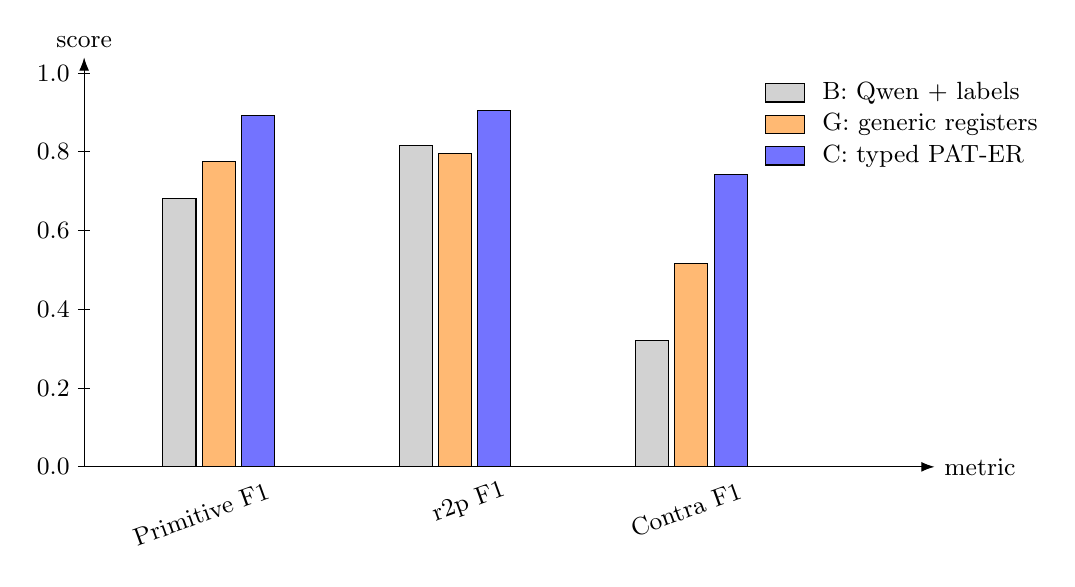
\begin{tikzpicture}[font=\small, >=Latex]
  \draw[->] (0,0) -- (10.8,0) node[right]{metric};
  \draw[->] (0,0) -- (0,5.2) node[above]{score};
  \foreach \y/\lab in {0/0.0,1/0.2,2/0.4,3/0.6,4/0.8,5/1.0}
    {\draw (-0.08,\y) -- (0.08,\y) node[left=4pt]{\lab};}

  % scale: score * 5
  \foreach \x/\name/\b/\g/\c in {
    1.0/Primitive F1/3.41/3.88/4.46,
    4.0/r2p F1/4.08/3.98/4.53,
    7.0/Contra F1/1.60/2.58/3.71
  }{
    \draw[fill=gray!35] (\x,0) rectangle ++(0.42,\b);
    \draw[fill=orange!55] (\x+0.5,0) rectangle ++(0.42,\g);
    \draw[fill=blue!55] (\x+1.0,0) rectangle ++(0.42,\c);
    \node[rotate=20, anchor=east] at (\x+1.45,-0.25) {\name};
  }
  \node[fill=gray!35, draw, minimum width=5mm] at (8.9,4.75) {};
  \node[right] at (9.25,4.75) {B: Qwen + labels};
  \node[fill=orange!55, draw, minimum width=5mm] at (8.9,4.35) {};
  \node[right] at (9.25,4.35) {G: generic registers};
  \node[fill=blue!55, draw, minimum width=5mm] at (8.9,3.95) {};
  \node[right] at (9.25,3.95) {C: typed PAT-ER};
\end{tikzpicture}%
}
\caption{Contribution matrix graph. Generic learned registers improve some metrics over token pooling, but typed PAT-ER registers add a further gain, especially on the role-to-primitive and contradiction axes.}
\label{fig:contribution_matrix}
\end{figure}

\begin{table}[H]
\caption{Primary architecture result on shallow OWA validation data, eight seeds. CIs are paired bootstrap 95\% intervals for B to C deltas.\label{tab:architecture_matrix}}
\footnotesize
\begin{tabularx}{\textwidth}{@{}p{0.28\linewidth}p{0.18\linewidth}p{0.18\linewidth}p{0.15\linewidth}X@{}}
\toprule
\textbf{Metric} & \textbf{B: Qwen + labels} & \textbf{C: PAT-ER registers} & \textbf{Delta} & \textbf{95\% CI} \\
\midrule
Primitive macro-F1 & 0.682 $\pm$ 0.027 & \textbf{0.891 $\pm$ 0.022} & \textbf{+0.209} & [0.182, 0.237] \\
Role-to-primitive macro-F1 & 0.815 $\pm$ 0.005 & \textbf{0.905 $\pm$ 0.029} & \textbf{+0.090} & [0.074, 0.110] \\
Contradiction recall & 0.242 $\pm$ 0.110 & \textbf{0.735 $\pm$ 0.202} & +0.492 & [0.280, 0.705] \\
Entailment refuted recall & 0.021 $\pm$ 0.059 & \textbf{0.427 $\pm$ 0.433} & +0.406 & [0.167, 0.677] \\
LM loss & 2.563 $\pm$ 0.059 & 2.555 $\pm$ 0.057 & $\approx$0 & not material \\
\bottomrule
\end{tabularx}
\end{table}


\begin{table}[H]
\caption{Paired seed deltas for the structured-state control. Bold entries have bootstrap 95\% confidence intervals excluding zero. The G $\rightarrow$ C rows test whether typed PAT-ER flow improves over generic learned registers.\label{tab:reviewer_deltas}}
\scriptsize
\resizebox{\textwidth}{!}{%
\begin{tabular}{@{}llllll@{}}
\toprule
\textbf{Delta} & \textbf{Primitive macro-F1} & \textbf{R2P macro-F1} & \textbf{Contradiction recall} & \textbf{Contradiction F1} & \textbf{Entailment-refuted recall} \\
\midrule
B $\rightarrow$ G, shallow & \textbf{+0.094 [0.060, 0.130]} & $-0.020$ [$-0.062$, 0.020] & \textbf{+0.188 [0.023, 0.364]} & \textbf{+0.195 [0.072, 0.316]} & +0.073 [$-0.062$, 0.281] \\
G $\rightarrow$ C, shallow & \textbf{+0.116 [0.080, 0.151]} & \textbf{+0.110 [0.064, 0.160]} & \textbf{+0.273 [0.148, 0.398]} & \textbf{+0.227 [0.099, 0.380]} & +0.333 [$-0.031$, 0.688] \\
B $\rightarrow$ C, shallow & \textbf{+0.209 [0.182, 0.237]} & \textbf{+0.091 [0.074, 0.110]} & \textbf{+0.460 [0.278, 0.636]} & \textbf{+0.422 [0.277, 0.561]} & \textbf{+0.406 [0.167, 0.677]} \\
G $\rightarrow$ C, deep/CWA & \textbf{+0.097 [0.070, 0.125]} & \textbf{+0.091 [0.048, 0.136]} & \textbf{+0.307 [0.182, 0.420]} & \textbf{+0.245 [0.146, 0.354]} & \textbf{+0.398 [0.057, 0.761]} \\
\bottomrule
\end{tabular}%
}
\end{table}


The role-to-primitive contradiction axis is the clearest discriminator between
generic and typed structure. Generic registers are worse than token pooling on
role-to-primitive contradiction F1, while typed PAT-ER recovers it. In paired
seed deltas, B $\rightarrow$ G is negative on this axis ($-0.273$, 95\% CI
[$-0.443$, $-0.097$]), whereas G $\rightarrow$ C is strongly positive
(+0.483, 95\% CI [0.239, 0.733]). This indicates that undifferentiated register
capacity cannot substitute for typed event-role $\rightarrow$ primitive
coupling.

\subsection{Warm-Started Usable Model}

Condition C proves the architecture. Condition D is the usable model: it
retains much of the side-state behavior while reducing LM loss from 2.555 to
1.344. The warm-start sequence was not a single lucky tuning run. It required
four validated stages: frozen-backbone register learning, safe register-only
injection, upper-layer adapter opening, and KL-guarded top-layer adaptation.

\begin{figure}[H]
\centering
\resizebox{\textwidth}{!}{%
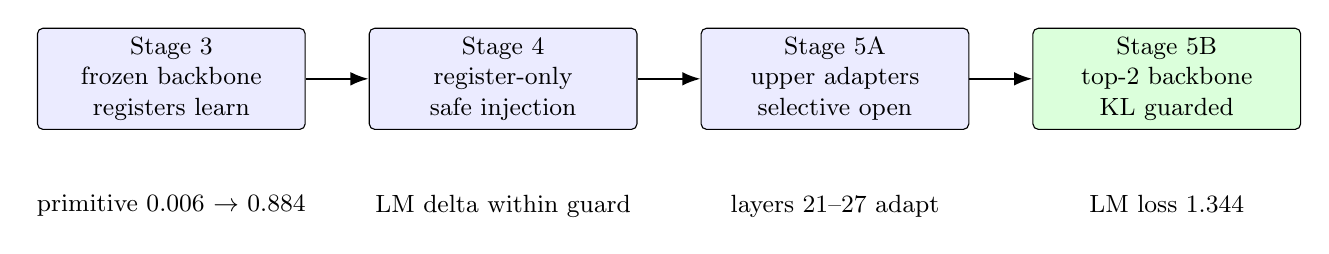
\begin{tikzpicture}[
  font=\small,
  >=Latex,
  stagebox/.style={draw, rounded corners=2pt, minimum width=34mm, minimum height=12mm, align=center, fill=blue!8},
  pass/.style={draw, rounded corners=2pt, minimum width=34mm, minimum height=12mm, align=center, fill=green!14},
  arr/.style={->, line width=0.8pt}
]
\node[stagebox] (s3) {Stage 3\\frozen backbone\\registers learn};
\node[stagebox, right=8mm of s3] (s4) {Stage 4\\register-only\\safe injection};
\node[stagebox, right=8mm of s4] (s5a) {Stage 5A\\upper adapters\\selective open};
\node[pass, right=8mm of s5a] (s5b) {Stage 5B\\top-2 backbone\\KL guarded};
\draw[arr] (s3) -- (s4);
\draw[arr] (s4) -- (s5a);
\draw[arr] (s5a) -- (s5b);
\node[below=7mm of s3] {primitive 0.006 $\to$ 0.884};
\node[below=7mm of s4] {LM delta within guard};
\node[below=7mm of s5a] {layers 21--27 adapt};
\node[below=7mm of s5b] {LM loss 1.344};
\end{tikzpicture}%
}
\caption{Warm-start validation sequence. The usable model is obtained only after safe injection, selective adapter opening, and KL-guarded top-layer adaptation.}
\label{fig:warmstart_stages}
\end{figure}

\begin{table}[H]
\caption{Warm-start validation stages.\label{tab:warmstart_stages}}
\footnotesize
\begin{tabularx}{\textwidth}{@{}p{0.16\linewidth}p{0.39\linewidth}X@{}}
\toprule
\textbf{Stage} & \textbf{What was tested} & \textbf{Key result} \\
\midrule
Stage 3 & Train PAT-ER registers on frozen Qwen3 backbone & Primitive macro-F1 0.006 to 0.884; LM unchanged \\
Stage 4 & Open safe register-only injection & LM delta within guard; KL below threshold; generation modulated \\
Stage 5A & Open upper-layer PAT-ER adapters & Layers 21--27 adapt; lower layers remain unchanged \\
Stage 5B & Unfreeze top two Qwen layers under KL guard & Backbone adapts safely; KL guard never triggers \\
\bottomrule
\end{tabularx}
\end{table}



\subsection{Decoupled Product Interface}

The first shared-layer interface SFT improved tool calls but damaged the
role-to-primitive bridge by 0.094. The accepted solution decouples product
generation from side-state measurement: train copied top decoder blocks only in
\texttt{interface\_mode}; keep base mode byte-identical to Condition D.

\begin{figure}[H]
\centering
\resizebox{0.9\textwidth}{!}{%
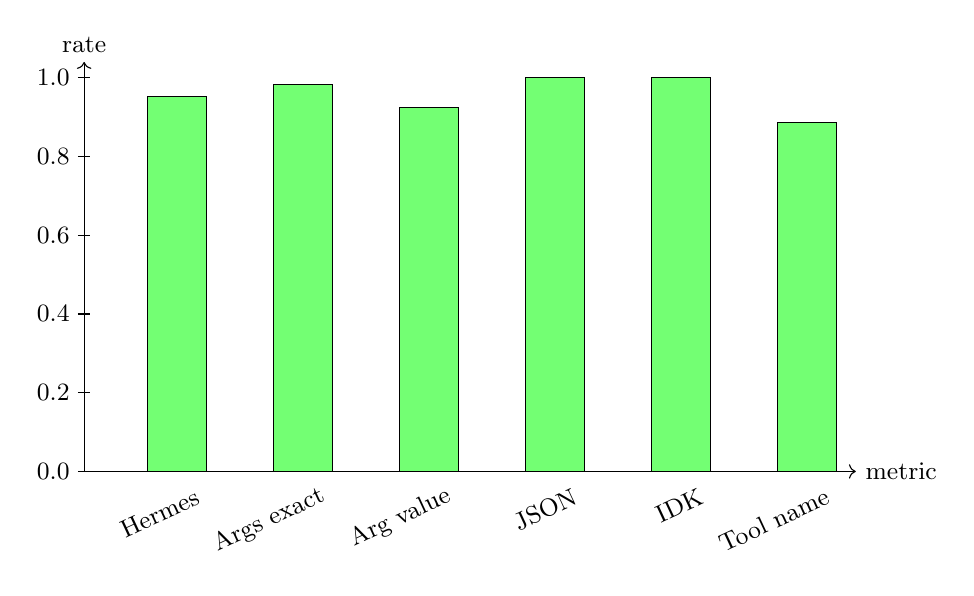
\begin{tikzpicture}[font=\small]
  \draw[->] (0,0) -- (9.8,0) node[right]{metric};
  \draw[->] (0,0) -- (0,5.2) node[above]{rate};
  \foreach \y/\lab in {0/0.0,1/0.2,2/0.4,3/0.6,4/0.8,5/1.0}
    {\draw (-0.08,\y) -- (0.08,\y) node[left=4pt]{\lab};}
  \foreach \x/\name/\val in {
    0.8/Hermes/4.76,
    2.4/Args exact/4.91,
    4.0/Arg value/4.62,
    5.6/JSON/5.00,
    7.2/IDK/5.00,
    8.8/Tool name/4.43
  }{
    \draw[fill=green!55] (\x,0) rectangle ++(0.75,\val);
    \node[rotate=25, anchor=east] at (\x+0.75,-0.25) {\name};
  }
\end{tikzpicture}%
}
\caption{Decoupled interface metrics on 242 held-out prompts. Tool-name exact copying is the remaining boundary; schema-grounded calls, exact arguments, JSON, and IDK pass.}
\label{fig:interface_metrics}
\end{figure}


\begin{table}[H]
\caption{Decoupled interface evaluation on 242 held-out prompts, three seeds.\label{tab:interface_eval}}
\footnotesize
\begin{tabularx}{\textwidth}{@{}p{0.34\linewidth}p{0.18\linewidth}p{0.16\linewidth}X@{}}
\toprule
\textbf{Metric} & \textbf{Result} & \textbf{Target} & \textbf{Verdict} \\
\midrule
Hermes parse & \textbf{0.952} & $\ge$0.90 & Pass \\
Tool arguments exact & \textbf{0.981} & $\ge$0.80 & Pass \\
Argument value accuracy & 0.923 & -- & Reported \\
JSON valid / required keys & \textbf{1.000 / 1.000} & $\ge$0.95 & Pass \\
IDK precision/recall/F1 & \textbf{1.000} & 1.000 & Pass \\
Base-mode primitive/r2p/LM vs D & byte-identical & exact & Pass \\
Tool-name exact accuracy & 0.886 & $\ge$0.90 & Boundary \\
\bottomrule
\end{tabularx}
\end{table}



On 242 held-out prompts across three seeds, the decoupled interface reaches
Hermes parse 0.952, exact argument correctness 0.981, JSON validity 1.000, and
IDK F1 1.000. Exact unseen tool-name copying remains imperfect at 0.886. This is
reported as an interface limit, not as a side-state regression, because base
mode is identical to Condition D.

\subsection{Negative Results}

The negative result record is central to the claim because it shows that the
reported path is not merely the last surviving configuration. Several plausible
alternatives failed for diagnosed reasons.

\begin{figure}[H]
\centering
\resizebox{\textwidth}{!}{%
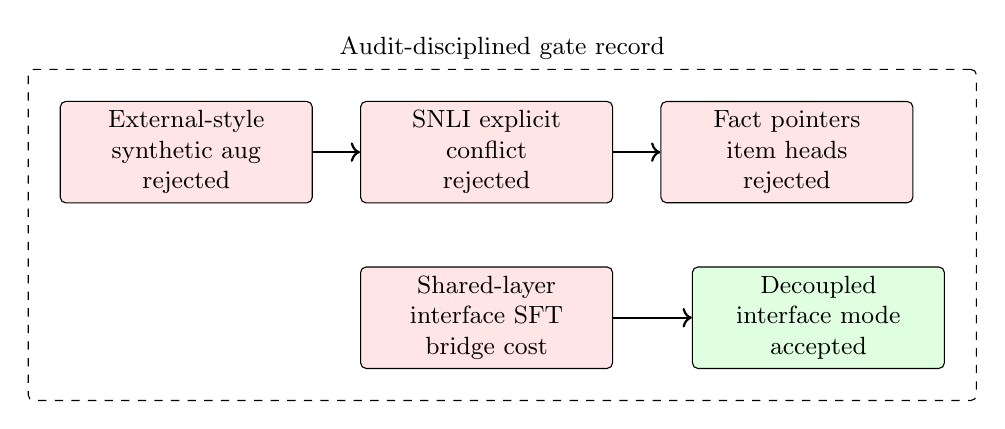
\begin{tikzpicture}[
  font=\small,
  bad/.style={draw, rounded corners=2pt, minimum width=32mm, minimum height=10mm, align=center, fill=red!10},
  good/.style={draw, rounded corners=2pt, minimum width=32mm, minimum height=10mm, align=center, fill=green!12},
  arr/.style={->, line width=0.8pt}
]
\node[bad] (a) {External-style\\synthetic aug\\rejected};
\node[bad, right=6mm of a] (b) {SNLI explicit\\conflict\\rejected};
\node[bad, right=6mm of b] (c) {Fact pointers\\item heads\\rejected};
\node[bad, below=8mm of b] (d) {Shared-layer\\interface SFT\\bridge cost};
\node[good, right=10mm of d] (e) {Decoupled\\interface mode\\accepted};
\draw[arr] (a) -- (b);
\draw[arr] (b) -- (c);
\draw[arr] (d) -- (e);
\node[draw, dashed, rounded corners=2pt, fit=(a)(b)(c)(d)(e), inner sep=4mm,
      label={[font=\small]above:Audit-disciplined gate record}] {};
\end{tikzpicture}%
}
\caption{Negative-result map. Plausible additions were tested and rejected when they harmed the targeted slice or damaged the bridge.}
\label{fig:negative_results}
\end{figure}


\begin{table}[H]
\caption{Documented negative results and retained decision.\label{tab:negative_results}}
\footnotesize
\begin{tabularx}{\textwidth}{@{}p{0.25\linewidth}p{0.38\linewidth}X@{}}
\toprule
\textbf{Gate} & \textbf{Observed failure} & \textbf{Decision} \\
\midrule
Synthetic external-style augmentation & Hurt the real external slice even when synthetic-ext spans were learnable & Do not merge; use only for eval/curriculum \\
SNLI / explicit-conflict NLI & Improved its own conflict form but damaged ProofWriter contradiction & Reject from main mix \\
Token fact pointers & Failed to learn distributed fact sets and regressed MP & Gate off \\
Evidence-item heads & Supporting item learned weakly; contradicting item did not learn & Gate off \\
Deep/CWA from-scratch data & Improved in-distribution deep/CWA but destroyed shallow contradiction & Do not merge for 450M-from-scratch \\
Stage 6B aux-refresh & Catastrophic forgetting of contingency and axiom boundaries & Reject E \\
Shared-layer interface SFT & Tool calls improved but role-to-primitive regressed by 0.094 & Replace with decoupled interface mode \\
\bottomrule
\end{tabularx}
\end{table}



The pattern is consistent. Synthetic substitutes for real external data hurt
the real external slice. Explicit-conflict NLI helps its own surface
contradiction but hurts ProofWriter contradiction. Fact-level pointer heads do
not help at the available refutation density. Aux-refresh on the adapted
backbone causes class forgetting. Shared-layer SFT improves output formatting
but damages the bridge. The accepted recipe avoids these failure modes by
keeping architecture measurement and product generation decoupled.

\section{Discussion}
\label{sec:discussion}

\subsection{Logical Primitives as Semantic Heads}

The evidence supports the view that logical primitives can be operationalized as
semantic heads. The primitive stream is not a symbolic theorem prover. It is a
fixed latent interface that forces the model to answer different semantic
questions with different state channels. This matters because many reasoning
failures are not simply failures to produce the right text; they are failures to
separate the kind of answer being produced.

The strongest support is the B/G/C ladder. All three conditions share the same
Qwen3-0.6B backbone, data, and supervised labels. B has access to labels through
token-pooled auxiliary heads. G adds learned registers but removes typed
event-role-to-primitive organization. C restores the typed PAT-ER flow. The
consistent G-to-C gain means that the result is not explained merely by label
availability or by adding generic latent state.

\subsection{Fixed Flow Versus Flexible Generation}

The answer to whether the approach can be used as fixed flow is: yes, but only
where the flow is treated as semantic state, not as a complete reasoning engine.
The fixed flow is:

\begin{equation}
\text{tokens}
\rightarrow
\text{event roles}
\rightarrow
\text{primitive registers}
\rightarrow
\text{support/IDK/tool/interface decisions}.
\label{eq:semantic_flow}
\end{equation}

This flow is useful because it is ablatable and measurable. Removing registers
or replacing them with token-pooled heads changes the result. However, deep
closed-world refutation remains difficult, and the model should not be described
as solving theorem proving.

\subsection{Why Warm-Start Changed the Strategy}

The 450M-from-scratch track was valuable because it exposed the right data and
label structure. It also reached a reasoning ceiling. Warm-starting from
Qwen3-0.6B changed the regime: the pretrained decoder supplies language
competence, while PAT-ER supplies explicit semantic side-state. The safe
modulation rule--register-only fusion, detached fuse input, injection-only
training, and very small injection learning rate--is therefore not an
implementation detail; it is the condition under which side-state can attach to
a pretrained decoder without damaging it.

\subsection{Usability Requires Decoupling}

The product interface result shows that architecture evidence and interface
behavior should not share all adaptation capacity. Shared-layer SFT created a
direct conflict: it made tool calls better but damaged the role-to-primitive
bridge. Mode-gated interface layers solve this by making output behavior a
separate execution path. This is a practical design rule for usable systems:
measure side-state in base mode; generate product-format outputs in
\texttt{interface\_mode}; never treat the two as interchangeable.

\section{Limitations}
\label{sec:limitations}

PAT-ER proposes and predicts; it does not prove, certify, or guarantee.

First, the reasoning datasets are narrow. ProofWriter and FOLIO are appropriate
for controlled logical supervision, but they do not cover broad real-world
reasoning. Second, deep/CWA refutation remains a known limit. Warm-started
registers exceed the from-scratch 450M ceiling, but contradiction recall is not
perfect. Third, the usable interface is not safety-certified. Tool calls are
proposals and must be validated against a real schema before execution. Fourth,
unseen tool-name exact accuracy is 0.886, below the exact-name target of 0.90.
The failures are semantic substitution and multi-token truncation on a minority
of unseen names. Fifth, 760M-from-scratch is not validated; the validated usable
path is warm-started Qwen3-0.6B plus PAT-ER side-state and decoupled interface
mode.

The paper also does not claim that every logical primitive can be exhaustively
captured by a fixed neural head. The claim is narrower: selected primitive
families can be treated as semantic heads well enough to produce measurable
architecture signal and usable guarded output.


\section{Conclusions}
\label{sec:conclusions}

PAT-ER tests a concrete hypothesis: logical primitives can function as semantic
heads in a decoder architecture when they are coupled to event-role registers
rather than inferred only from pooled token states or stored in generic learned
registers. The eight-seed B/G/C matrix supports this hypothesis. Relative to
token pooling, typed PAT-ER improves primitive macro-F1 by 0.209 and
role-to-primitive macro-F1 by 0.091 with no LM-loss cost on the same pretrained
backbone. Relative to generic registers, it adds +0.116 primitive macro-F1 and
+0.110 role-to-primitive macro-F1, showing that typed flow matters beyond
undifferentiated latent capacity.

The usable-model path is also established but bounded. Warm-started PAT-ER
recovers pretrained LM quality, safe register-only modulation preserves the
decoder, and decoupled interface mode yields robust schema-grounded function
calling and JSON output at zero measured side-state cost. The model is not a
theorem prover, not production safety-certified, and not a perfect tool-name
copying system. Its contribution is a measured, ablatable semantic side-state
and a practical way to use it without damaging the base language model.

\vspace{6pt}

\authorcontributions{Conceptualization, N.K.\ and M.M.; methodology, N.K.; software, N.K.; validation, N.K.\ and M.M.; formal analysis, N.K.; investigation, N.K.; data curation, N.K.; writing---original draft preparation, N.K.; writing---review and editing, N.K.\ and M.M.; visualization, N.K.; supervision, M.M.; project administration, M.M.; funding acquisition, M.M. All authors have read and agreed to the published version of the manuscript.}

\funding{This research was funded by the Ministry of Science and Higher Education of the Republic of Kazakhstan, grant number BR24993001, ``Creation of a large language model (LLM) to maintain the implementation of Kazakh language and increase the technological progress''.}

\institutionalreview{Not applicable. This work uses synthetic data and publicly released research datasets under their stated licenses. No new human-subjects data was collected.}

\informedconsent{Not applicable.}

\dataavailability{The manuscript source, model code, configuration files, conversion scripts, evaluation scripts, and result-summary records are maintained in the accompanying project repository. Converted datasets and trained checkpoints are stored outside the manuscript source because they require separate storage and upstream-license review before redistribution. The reported tables are derived from retained evaluation records. Running new inference with the usable interface model additionally requires the warm-start/interface checkpoint files, which can be provided to editors and reviewers through controlled access under the applicable model and dataset licenses.}

\acknowledgments{The authors gratefully acknowledge support from the Ministry of Science and Higher Education of the Republic of Kazakhstan, and computational resources provided by Al-Farabi Kazakh National University.}

\conflictsofinterest{The authors declare no conflicts of interest. The funders had no role in the design of the study; in the collection, analyses, or interpretation of data; in the writing of the manuscript; or in the decision to publish the results.}


\FloatBarrier
\reftitle{References}
\bibliography{refs}

\end{document}
